\section{附录：参数表数据示例和Demo截图}\label{sec:appendix}
\subsection{参数表数据示例}
{\scriptsize
\begin{verbatim}
{
  "recordId": "2090346294581600257",
  "modelId": "3d7a135894fa",
  "modelFileName": "仿真云平台测试专用-v0.2-0820-1539.fs",
  "status": "RUNNING",
  "snapshotAt": 1787212506689,
  "mcpTableName": "MCP",
  "mcpTableFound": true,
  "mcpRows": [
    {
      "rowIndex": 0,
      "tableName": ".订单表",
      "remark": "",
      "exists": true,
      "tableId": "8eca1be7b67e",
      "wholeNo": ".订单表",
      "rowCount": 2,
      "columnCount": 5
    },
    {
      "rowIndex": 1,
      "tableName": ".工站参数",
      "remark": "",
      "exists": true,
      "tableId": "9138d214d65e",
      "wholeNo": ".工站参数",
      "rowCount": 7,
      "columnCount": 9
    },
    {
      "rowIndex": 2,
      "tableName": ".不良品记录表",
      "remark": "Out",
      "exists": true,
      "tableId": "8a24b7d28089",
      "wholeNo": ".不良品记录表",
      "rowCount": 18,
      "columnCount": 5
    }
  ],
  "tables": [
    {
      "tableId": "8eca1be7b67e",
      "tableName": "订单表",
      "wholeNo": ".订单表",
      "remark": "",
      "columnCount": 5,
      "rowCount": 2,
      "columns": [
        {
          "index": 0,
          "name": "MU类型",
          "type": "String",
          "format": "General",
          "width": 84,
          "indexColumn": false
        },
        {
          "index": 1,
          "name": "名称",
          "type": "String",
          "format": "General",
          "width": 153,
          "indexColumn": false
        },
        {
          "index": 2,
          "name": "数量",
          "type": "Int",
          "format": "General",
          "width": 120,
          "indexColumn": false
        },
        {
          "index": 3,
          "name": "创建时间",
          "type": "Time",
          "format": "dd:hh:mm:ss.SSS",
          "width": 160,
          "indexColumn": false
        },
        {
          "index": 4,
          "name": "优先级",
          "type": "Int",
          "format": "General",
          "width": 100,
          "indexColumn": false
        }
      ],
      "rows": [
        [
          "PartA",
          "汽车门锁总成A",
          "80",
          "0",
          "0"
        ],
        [
          "PartB",
          "汽车门锁总成B",
          "20",
          "0",
          "0"
        ]
      ]
    },
    {
      "tableId": "9138d214d65e",
      "tableName": "工站参数",
      "wholeNo": ".工站参数",
      "remark": "",
      "columnCount": 9,
      "rowCount": 7,
      "columns": [
        {
          "index": 0,
          "name": "工站",
          "type": "String",
          "format": "General",
          "width": 100,
          "indexColumn": false
        },
        {
          "index": 1,
          "name": "加工时长",
          "type": "String",
          "format": "General",
          "width": 228,
          "indexColumn": false
        },
        {
          "index": 2,
          "name": "加工合格率",
          "type": "String",
          "format": "General",
          "width": 100,
          "indexColumn": false
        },
        {
          "index": 3,
          "name": "MTBF",
          "type": "String",
          "format": "General",
          "width": 100,
          "indexColumn": false
        },
        {
          "index": 4,
          "name": "MTTR",
          "type": "String",
          "format": "General",
          "width": 100,
          "indexColumn": false
        },
        {
          "index": 5,
          "name": "换型",
          "type": "String",
          "format": "General",
          "width": 100,
          "indexColumn": false
        },
        {
          "index": 6,
          "name": "返修成功率",
          "type": "String",
          "format": "General",
          "width": 100,
          "indexColumn": false
        },
        {
          "index": 7,
          "name": "最多返修次",
          "type": "String",
          "format": "General",
          "width": 100,
          "indexColumn": false
        },
        {
          "index": 8,
          "name": "工人",
          "type": "String",
          "format": "General",
          "width": 100,
          "indexColumn": false
        }
      ],
      "rows": [
        [
          ".预装",
          "Triangular(40,45,50)",
          "0.99",
          "不适用",
          "不适用",
          "不适用",
          "不适用",
          "不适用",
          "工人1"
        ],
        [
          ".压装",
          "Triangular(60,65,72)",
          "不适用",
          "7200",
          "600",
          "300",
          "不适用",
          "不适用",
          "工人2"
        ],
        [
          ".锁付1",
          "Triangular(32,35,40)",
          "0.995",
          "不适用",
          "不适用",
          "不适用",
          "不适用",
          "不适用",
          "工人3"
        ],
        [
          ".锁付2",
          "Triangular(32,35,40)",
          "0.995",
          "不适用",
          "不适用",
          "不适用",
          "不适用",
          "不适用",
          "工人3"
        ],
        [
          ".电检",
          "Triangular(65,70,78)",
          "0.95",
          "不适用",
          "不适用",
          "不适用",
          "不适用",
          "不适用",
          "工人4"
        ],
        [
          ".包装",
          "Triangular(36,40,45)",
          "不适用",
          "不适用",
          "不适用",
          "不适用",
          "不适用",
          "不适用",
          "工人4"
        ],
        [
          ".返修工位",
          "Triangular(100,120,150)",
          "不适用",
          "不适用",
          "不适用",
          "不适用",
          "0.90",
          "1",
          "工人5"
        ]
      ]
    },
    {
      "tableId": "8a24b7d28089",
      "tableName": "不良品记录表",
      "wholeNo": ".不良品记录表",
      "remark": "Out",
      "columnCount": 5,
      "rowCount": 18,
      "columns": [
        {
          "index": 0,
          "name": "MU编号",
          "type": "String",
          "format": "General",
          "width": 75,
          "indexColumn": false
        },
        {
          "index": 1,
          "name": "检测时间",
          "type": "Time",
          "format": "dd:hh:mm:ss.SSS",
          "width": 179,
          "indexColumn": false
        },
        {
          "index": 2,
          "name": "加工合计率",
          "type": "double",
          "format": "General",
          "width": 75,
          "indexColumn": false
        },
        {
          "index": 3,
          "name": "加工质量随机数",
          "type": "double",
          "format": "General",
          "width": 224,
          "indexColumn": false
        },
        {
          "index": 4,
          "name": "检验站",
          "type": "String",
          "format": "General",
          "width": 75,
          "indexColumn": false
        }
      ],
      "rows": [
        [
          "1000006",
          "48:40.493",
          "0.95",
          "0.9839332611759481",
          ".电检"
        ],
        [
          "1000009",
          "54:10.718",
          "0.95",
          "0.9608330859226331",
          ".电检"
        ],
        [
          "1000018",
          "1:13:42.089",
          "0.95",
          "0.9952906684597524",
          ".电检"
        ],
        [
          "1000028",
          "1:32:35.744",
          "0.95",
          "0.9585777662984521",
          ".电检"
        ],
        [
          "1000067",
          "3:0:56.783",
          "0.95",
          "0.966219510771312",
          ".电检"
        ],
        [
          "1000077",
          "3:22:25.714",
          "0.95",
          "0.9813904424209212",
          ".电检"
        ],
        [
          "1000077",
          "3:25:55.053",
          "0.95",
          "0.9621168485921084",
          ".电检"
        ],
        [
          "1000081",
          "3:35:10.087",
          "0.95",
          "0.989885938676186",
          ".电检"
        ],
        [
          "1000103",
          "4:51:15.709",
          "0.95",
          "0.9905912266541431",
          ".电检"
        ],
        [
          "1000121",
          "5:37:23.706",
          "0.95",
          "0.9959583392896706",
          ".电检"
        ],
        [
          "1000126",
          "5:47:14.148",
          "0.95",
          "0.9635888173821661",
          ".电检"
        ],
        [
          "1000147",
          "6:30:23.304",
          "0.95",
          "0.9601289268256603",
          ".电检"
        ],
        [
          "1000156",
          "6:49:38.077",
          "0.95",
          "0.9519641474721253",
          ".电检"
        ],
        [
          "1000159",
          "6:55:37.851",
          "0.95",
          "0.9737964161836378",
          ".电检"
        ],
        [
          "1000165",
          "7:8:27.625",
          "0.95",
          "0.9917270516743044",
          ".电检"
        ],
        [
          "1000199",
          "8:29:47.941",
          "0.95",
          "0.9535895423555071",
          ".电检"
        ],
        [
          "1000202",
          "8:41:9.328",
          "0.95",
          "0.9847126650417776",
          ".电检"
        ],
        [
          "1000204",
          "8:46:25.655",
          "0.95",
          "0.986009299767029",
          ".电检"
        ]
      ]
    }
  ],
  "missingTables": []
}    
\end{verbatim}
}\subsection{Demo程序的部分截图}
\begin{figure}[h!]
	\centering
	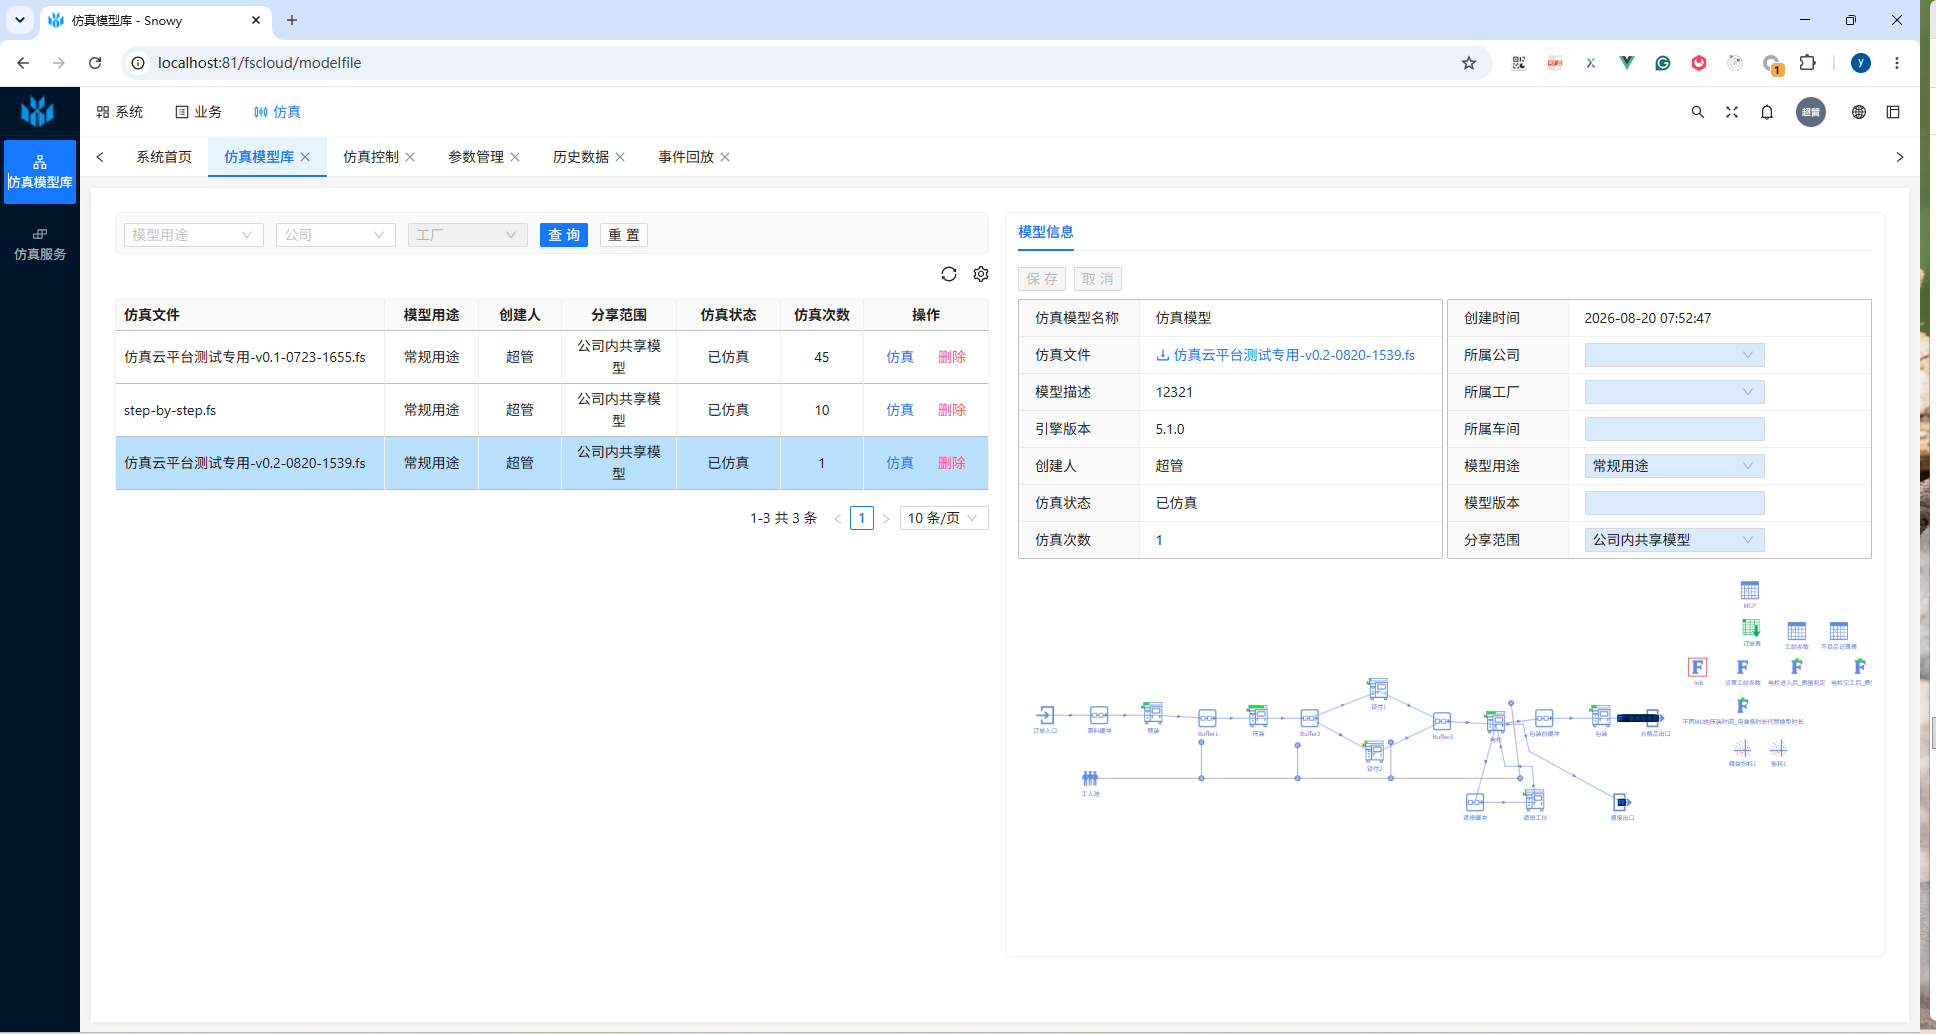
\includegraphics[width=0.9\textwidth]{pics/mcp/screen-model-lib.png}
	\caption{模型库}\label{fig:screen-model-lib}
\end{figure}
\begin{figure}[h!]
	\centering
	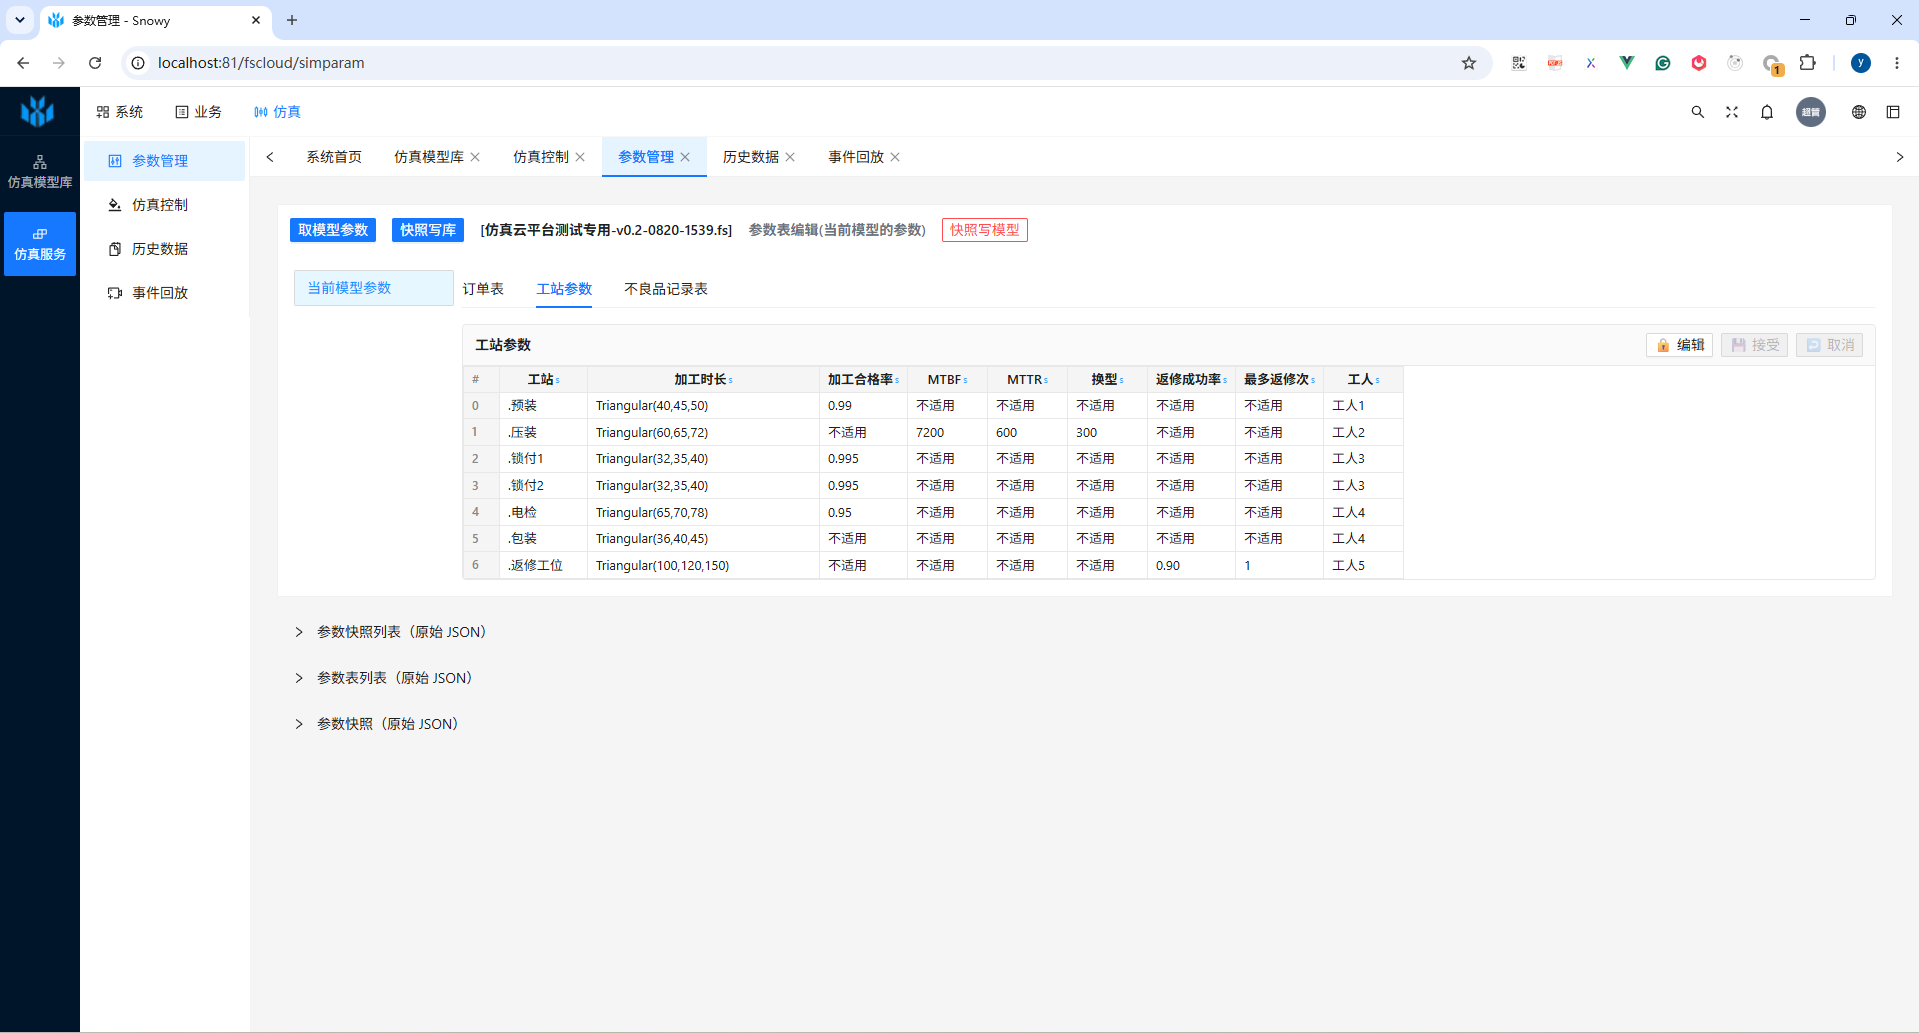
\includegraphics[width=0.9\textwidth]{pics/mcp/screen-param.png}
	\caption{参数表数据}\label{fig:screen-param}
\end{figure}
\begin{figure}[h!]
	\centering
	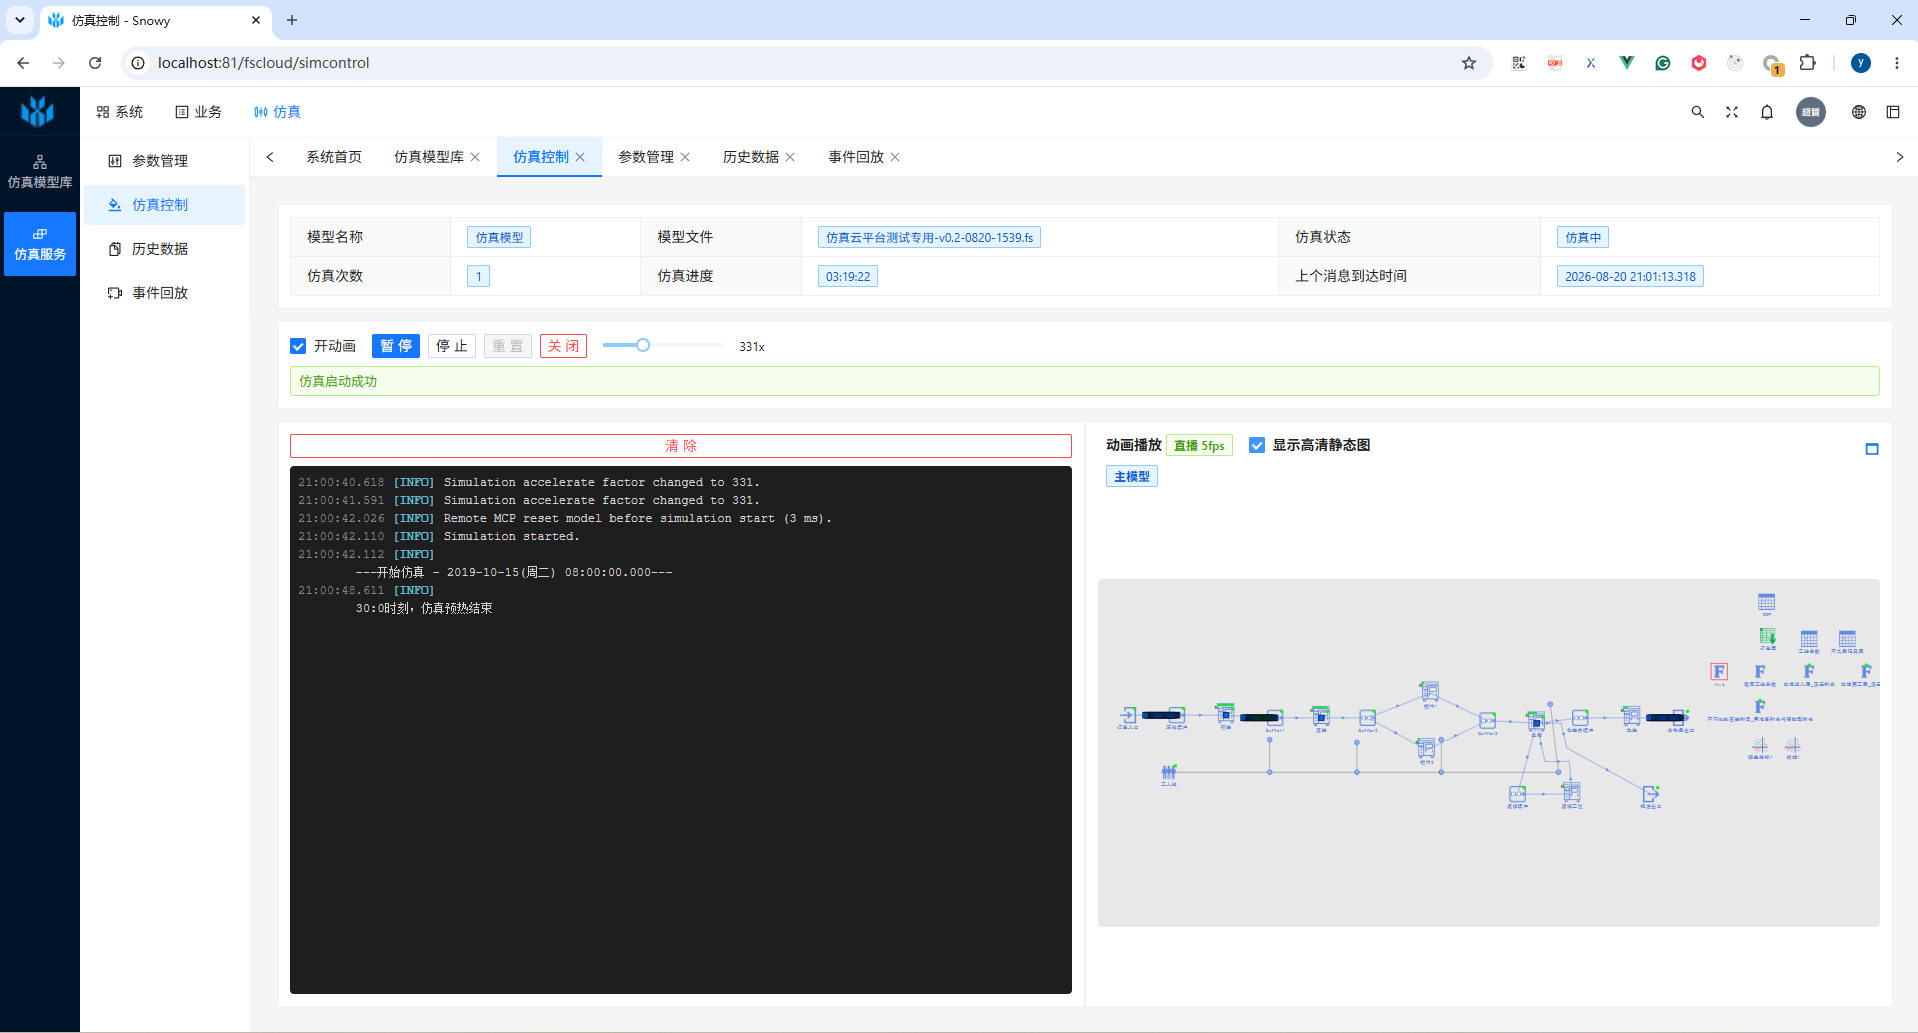
\includegraphics[width=0.9\textwidth]{pics/mcp/screen-sim-control.png}
	\caption{仿真控制}\label{fig:screen-sim-control}
\end{figure}
\begin{figure}[h!]
	\centering
	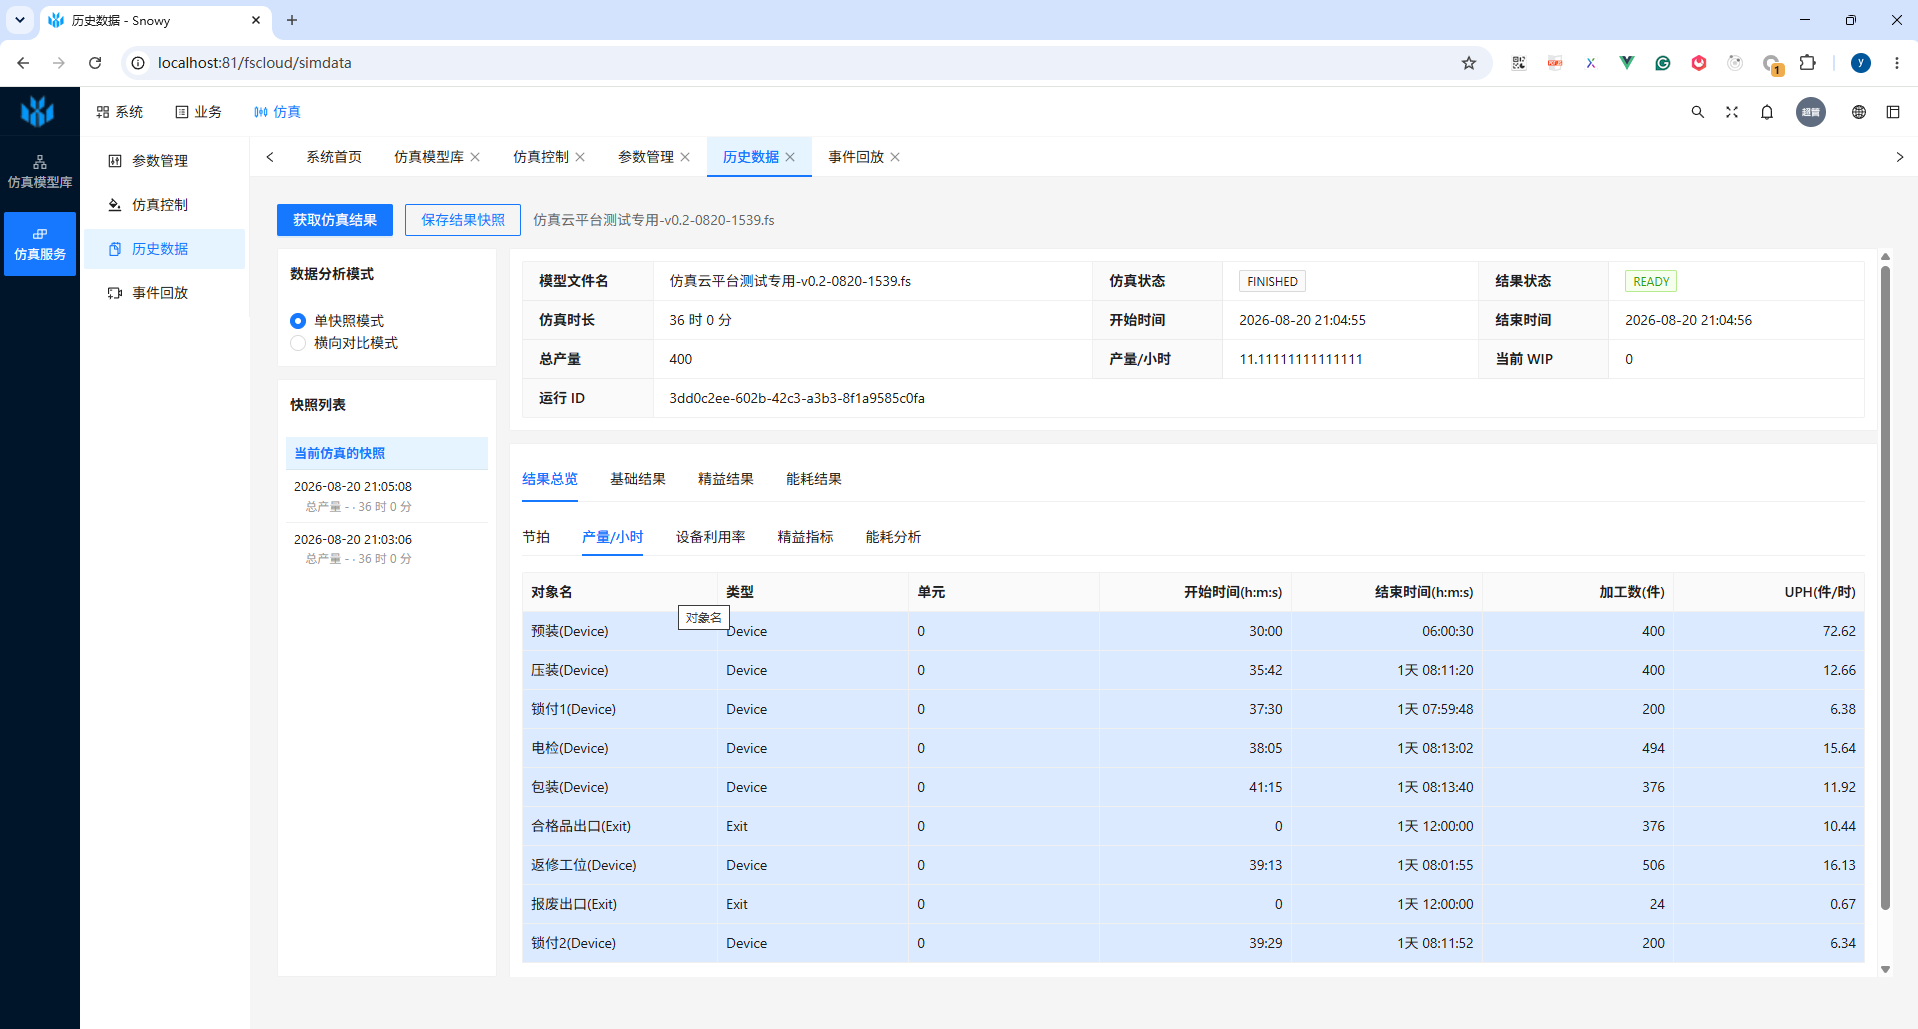
\includegraphics[width=0.9\textwidth]{pics/mcp/screen-sim-data-single.png}
	\caption{历史数据单快照查看}\label{fig:screen-sim-data-single}
\end{figure}
\begin{figure}[h!]
	\centering
	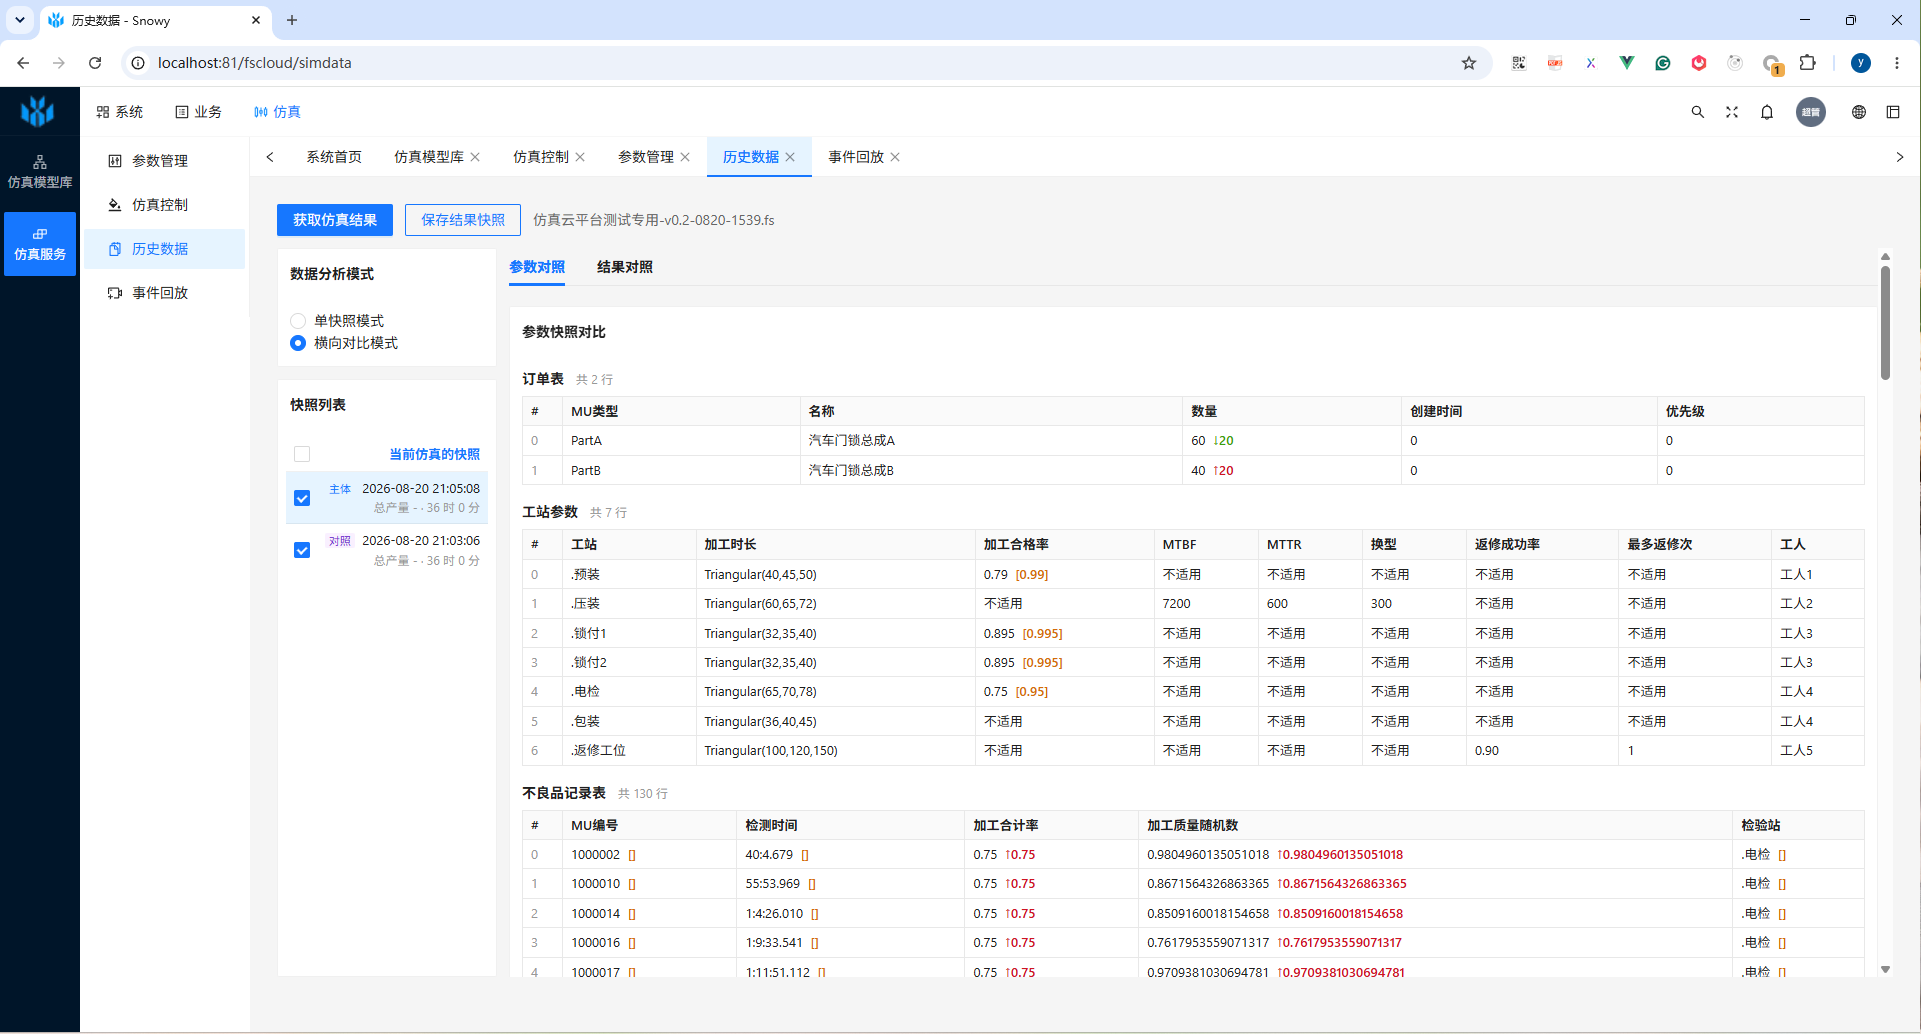
\includegraphics[width=0.9\textwidth]{pics/mcp/screen-sim-data-cmp-1.png}
	\caption{历史数据横向对比-参数}\label{fig:screen-sim-data-cmp-1}
\end{figure}
\begin{figure}[h!]
	\centering
	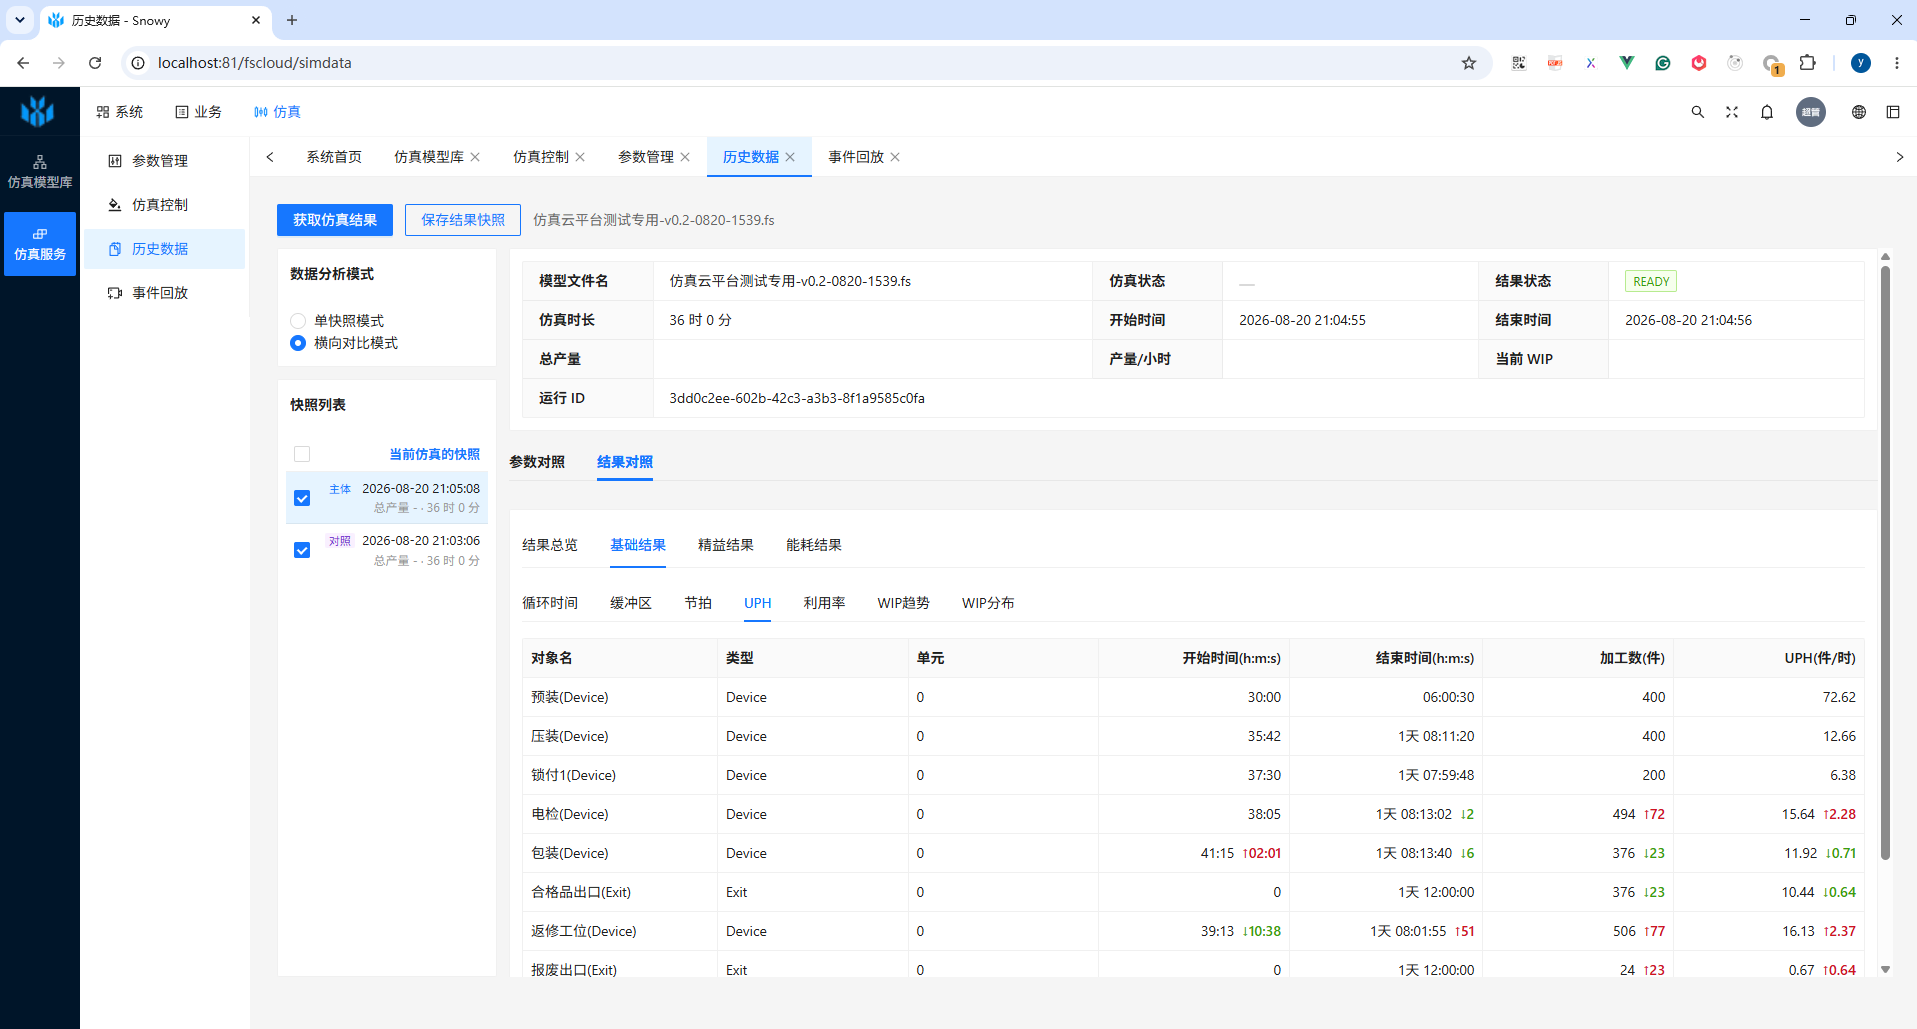
\includegraphics[width=0.9\textwidth]{pics/mcp/screen-sim-data-cmp-2.png}
	\caption{历史数据横向对比-仿真结果}\label{fig:screen-sim-data-cmp-2}
\end{figure}
\begin{figure}[h!]
	\centering
	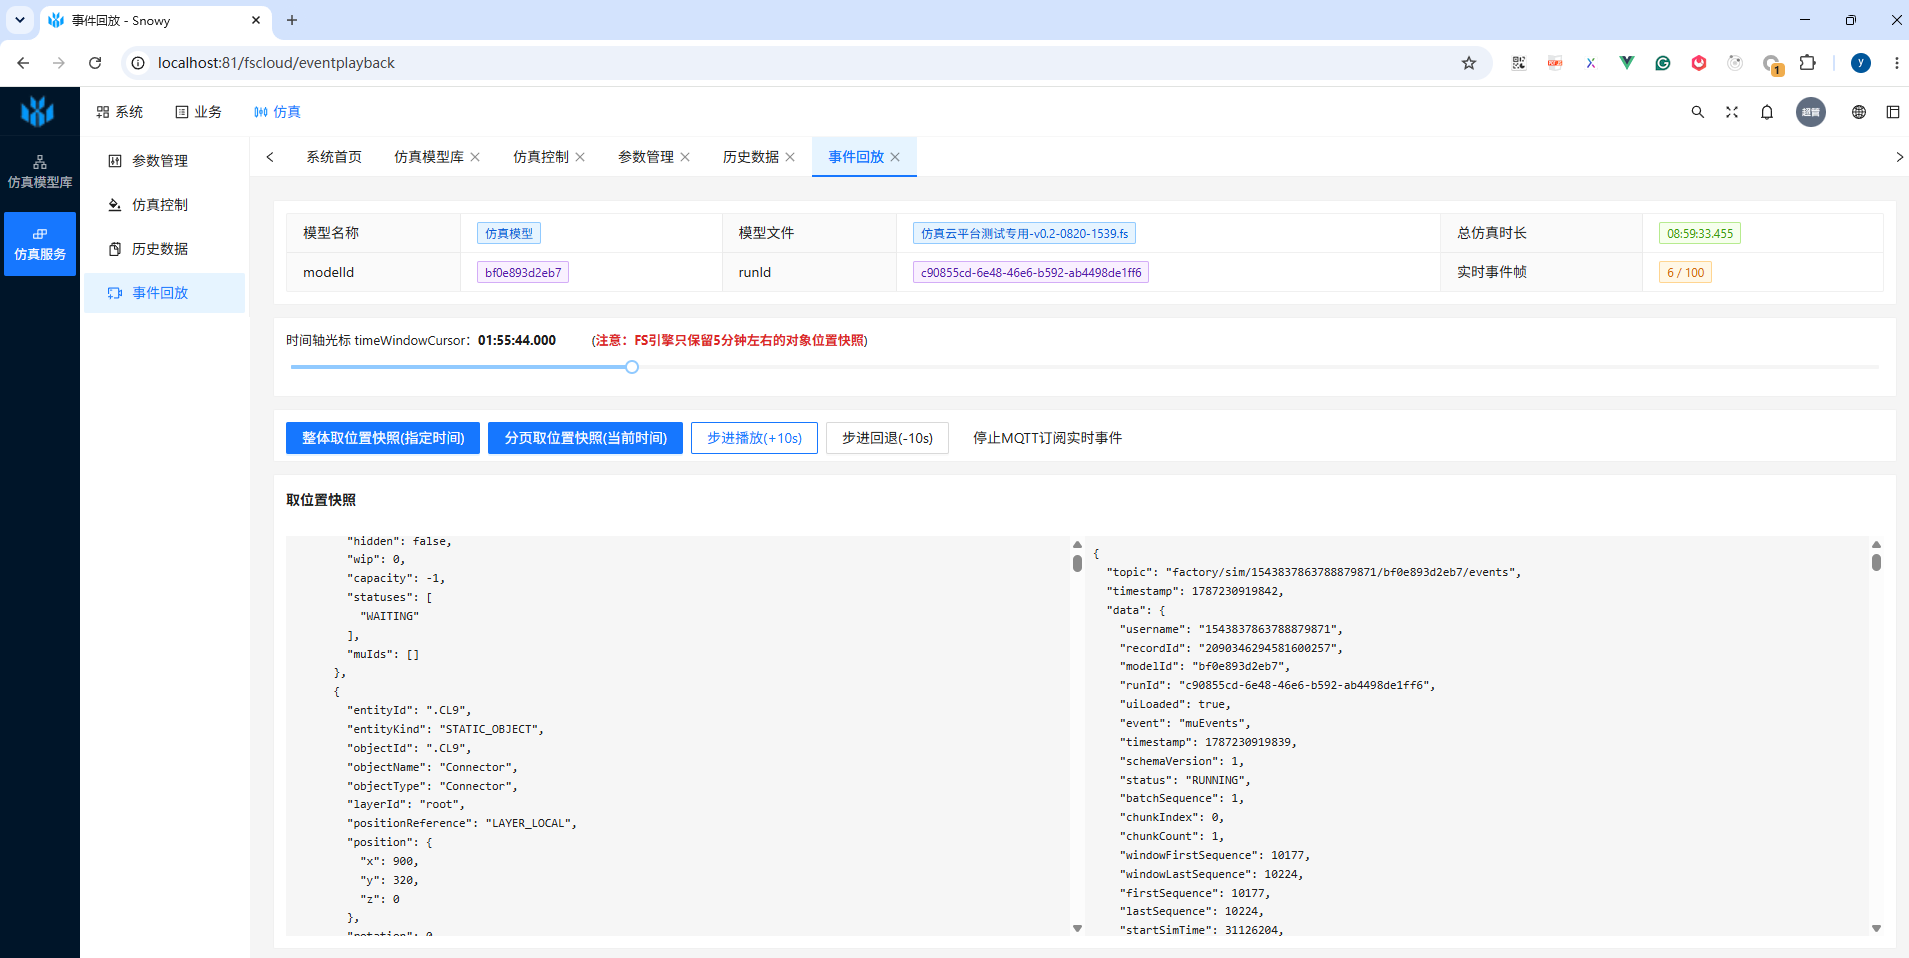
\includegraphics[width=0.9\textwidth]{pics/mcp/screen-event-playback.png}
	\caption{时间轴对象快照和事件回放}\label{fig:screen-event-playback}
\end{figure}

\section{附录：数据库相关表DDL}\label{appendix:database-ddl}
\subsection{模型库}
{\scriptsize
\begin{verbatim}
CREATE TABLE `fs_model_file` (
  `id` bigint NOT NULL AUTO_INCREMENT COMMENT '主键ID',
  `name` varchar(255) CHARACTER SET utf8mb4 COLLATE utf8mb4_unicode_ci NOT NULL COMMENT '仿真模型名称',
  `description` text CHARACTER SET utf8mb4 COLLATE utf8mb4_unicode_ci COMMENT '模型描述',
  `engine_version` varchar(32) CHARACTER SET utf8mb4 COLLATE utf8mb4_unicode_ci DEFAULT NULL COMMENT '引擎版本',
  `model_usage` varchar(128) CHARACTER SET utf8mb4 COLLATE utf8mb4_unicode_ci DEFAULT NULL COMMENT '模型用途',
  `user_id` bigint DEFAULT NULL COMMENT '创建人ID',
  `user_name` varchar(64) CHARACTER SET utf8mb4 COLLATE utf8mb4_unicode_ci DEFAULT NULL COMMENT '创建人名称',
  `image` varchar(512) CHARACTER SET utf8mb4 COLLATE utf8mb4_unicode_ci DEFAULT NULL COMMENT '预览图片路径/文件名',
  `model` varchar(512) CHARACTER SET utf8mb4 COLLATE utf8mb4_unicode_ci DEFAULT NULL COMMENT '模型文件路径/文件名',
  `model_company` varchar(255) CHARACTER SET utf8mb4 COLLATE utf8mb4_unicode_ci DEFAULT NULL COMMENT '模型所属公司',
  `model_factory` varchar(255) CHARACTER SET utf8mb4 COLLATE utf8mb4_unicode_ci DEFAULT NULL COMMENT '所属工厂',
  `model_warehouse` varchar(255) CHARACTER SET utf8mb4 COLLATE utf8mb4_unicode_ci DEFAULT NULL COMMENT '所属仓库',
  `model_version` varchar(255) CHARACTER SET utf8mb4 COLLATE utf8mb4_unicode_ci DEFAULT NULL COMMENT '模型版本',
  `share_flag` varchar(255) CHARACTER SET utf8mb4 COLLATE utf8mb4_unicode_ci DEFAULT '0' COMMENT '分享标注（见数据字典）',
  `created_at` datetime DEFAULT CURRENT_TIMESTAMP COMMENT '记录创建时间',
  `updated_at` datetime DEFAULT CURRENT_TIMESTAMP ON UPDATE CURRENT_TIMESTAMP COMMENT '记录更新时间',
  `sim_status` varchar(255) CHARACTER SET utf8mb4 COLLATE utf8mb4_0900_ai_ci NOT NULL DEFAULT 'SIM_STATUS_NOTYET' COMMENT '仿真状态',
  `sim_times` int NOT NULL DEFAULT '0' COMMENT '仿真次数',
  `model_id` varchar(255) CHARACTER SET utf8mb4 COLLATE utf8mb4_unicode_ci DEFAULT NULL COMMENT '模型ID（加载模型后生成）',
  PRIMARY KEY (`id`) USING BTREE,
  KEY `idx_user_id` (`user_id`) USING BTREE,
  KEY `idx_name` (`name`) USING BTREE,
  KEY `idx_model_company` (`model_company`) USING BTREE
) ENGINE=InnoDB AUTO_INCREMENT=2090346294581600258 DEFAULT CHARSET=utf8mb4 COLLATE=utf8mb4_unicode_ci ROW_FORMAT=DYNAMIC COMMENT='仿真模型文件表';    
\end{verbatim}
}

\subsection{参数快照}
{\scriptsize
\begin{verbatim}
CREATE TABLE `fs_sim_param_snapshot` (
  `ID` bigint NOT NULL AUTO_INCREMENT COMMENT '主键ID，自增',
  `MODEL_FILE_ID` varchar(64) CHARACTER SET utf8mb4 COLLATE utf8mb4_general_ci NOT NULL COMMENT '模型库记录ID（对应 MCP recordId）',
  `RUN_ID` varchar(64) CHARACTER SET utf8mb4 COLLATE utf8mb4_general_ci DEFAULT NULL COMMENT '仿真运行ID，NULL=单独落库，非NULL=与结果快照成对落库',
  `SNAPSHOT_AT` bigint NOT NULL COMMENT '快照时间（毫秒时间戳）',
  `PARAMETER_TABLES` json DEFAULT NULL COMMENT '参数表列表',
  `MCP_ROWS` json DEFAULT NULL COMMENT 'MCP 表中的参数表信息',
  `TABLES` json DEFAULT NULL COMMENT '各参数表内容（二维数组或对象数组）',
  `MISSING_TABLES` json DEFAULT NULL COMMENT '缺失的参数表列表',
  `CREATE_TIME` datetime DEFAULT NULL COMMENT '创建时间',
  `UPDATE_TIME` datetime DEFAULT NULL COMMENT '更新时间',
  PRIMARY KEY (`ID`) USING BTREE,
  KEY `IDX_FS_SIM_PARAM_SNAPSHOT_MODEL` (`MODEL_FILE_ID`) USING BTREE,
  KEY `IDX_FS_SIM_PARAM_SNAPSHOT_AT` (`MODEL_FILE_ID`,`SNAPSHOT_AT`) USING BTREE,
  KEY `IDX_FS_SIM_PARAM_SNAPSHOT_RUN` (`RUN_ID`)
) ENGINE=InnoDB AUTO_INCREMENT=11 DEFAULT CHARSET=utf8mb4 COLLATE=utf8mb4_general_ci ROW_FORMAT=DYNAMIC COMMENT='仿真参数快照';    
\end{verbatim}
}

\subsection{仿真结果数据快照}
{\scriptsize
\begin{verbatim}
CREATE TABLE `fs_sim_result_snapshot` (
  `ID` bigint NOT NULL AUTO_INCREMENT COMMENT '主键ID，自增',
  `RUN_ID` varchar(64) CHARACTER SET utf8mb4 COLLATE utf8mb4_general_ci NOT NULL COMMENT '仿真运行ID（MCP runId），唯一',
  `MODEL_FILE_ID` varchar(64) CHARACTER SET utf8mb4 COLLATE utf8mb4_general_ci NOT NULL COMMENT '模型库记录ID（MCP recordId）',
  `MODEL_FILE_NAME` varchar(255) CHARACTER SET utf8mb4 COLLATE utf8mb4_general_ci DEFAULT NULL COMMENT '模型文件名',
  `SIM_TIME` bigint DEFAULT NULL COMMENT '仿真总时长(毫秒)',
  `STARTED_AT` bigint DEFAULT NULL COMMENT '仿真开始时间戳(毫秒)',
  `FINISHED_AT` bigint DEFAULT NULL COMMENT '仿真结束时间戳(毫秒)',
  `RESULT_STATUS` varchar(32) CHARACTER SET utf8mb4 COLLATE utf8mb4_general_ci DEFAULT NULL COMMENT '结果状态(READY等)',
  `SNAPSHOT_AT` bigint DEFAULT NULL COMMENT '结果快照时间戳(毫秒)，落库/更新时间',
  `SUMMARY_RESULTS` json DEFAULT NULL COMMENT '总览结果(taktTime/uph/utilRate/leanMetrics/energyAnalysis)',
  `DATASETS` json DEFAULT NULL COMMENT '数据集元信息列表(名称/行数，不含数据)',
  `PART_CYCLE_TIME_FILE` varchar(255) CHARACTER SET utf8mb4 COLLATE utf8mb4_general_ci DEFAULT NULL COMMENT 'partCycleTime 数据文件名(大表落文件，相对路径)',
  `CREATE_TIME` datetime DEFAULT NULL COMMENT '创建时间',
  `UPDATE_TIME` datetime DEFAULT NULL COMMENT '更新时间',
  PRIMARY KEY (`ID`),
  UNIQUE KEY `UK_FS_SIM_RESULT_SNAPSHOT_RUN` (`RUN_ID`),
  KEY `IDX_FS_SIM_RESULT_SNAPSHOT_MODEL` (`MODEL_FILE_ID`,`SNAPSHOT_AT`)
) ENGINE=InnoDB AUTO_INCREMENT=8 DEFAULT CHARSET=utf8mb4 COLLATE=utf8mb4_general_ci COMMENT='仿真结果快照';    
\end{verbatim}
}

\section{附录：CherryStudio辅助调试}\label{appendix:cherry-studio}
\begin{figure}[h!]
	\centering
	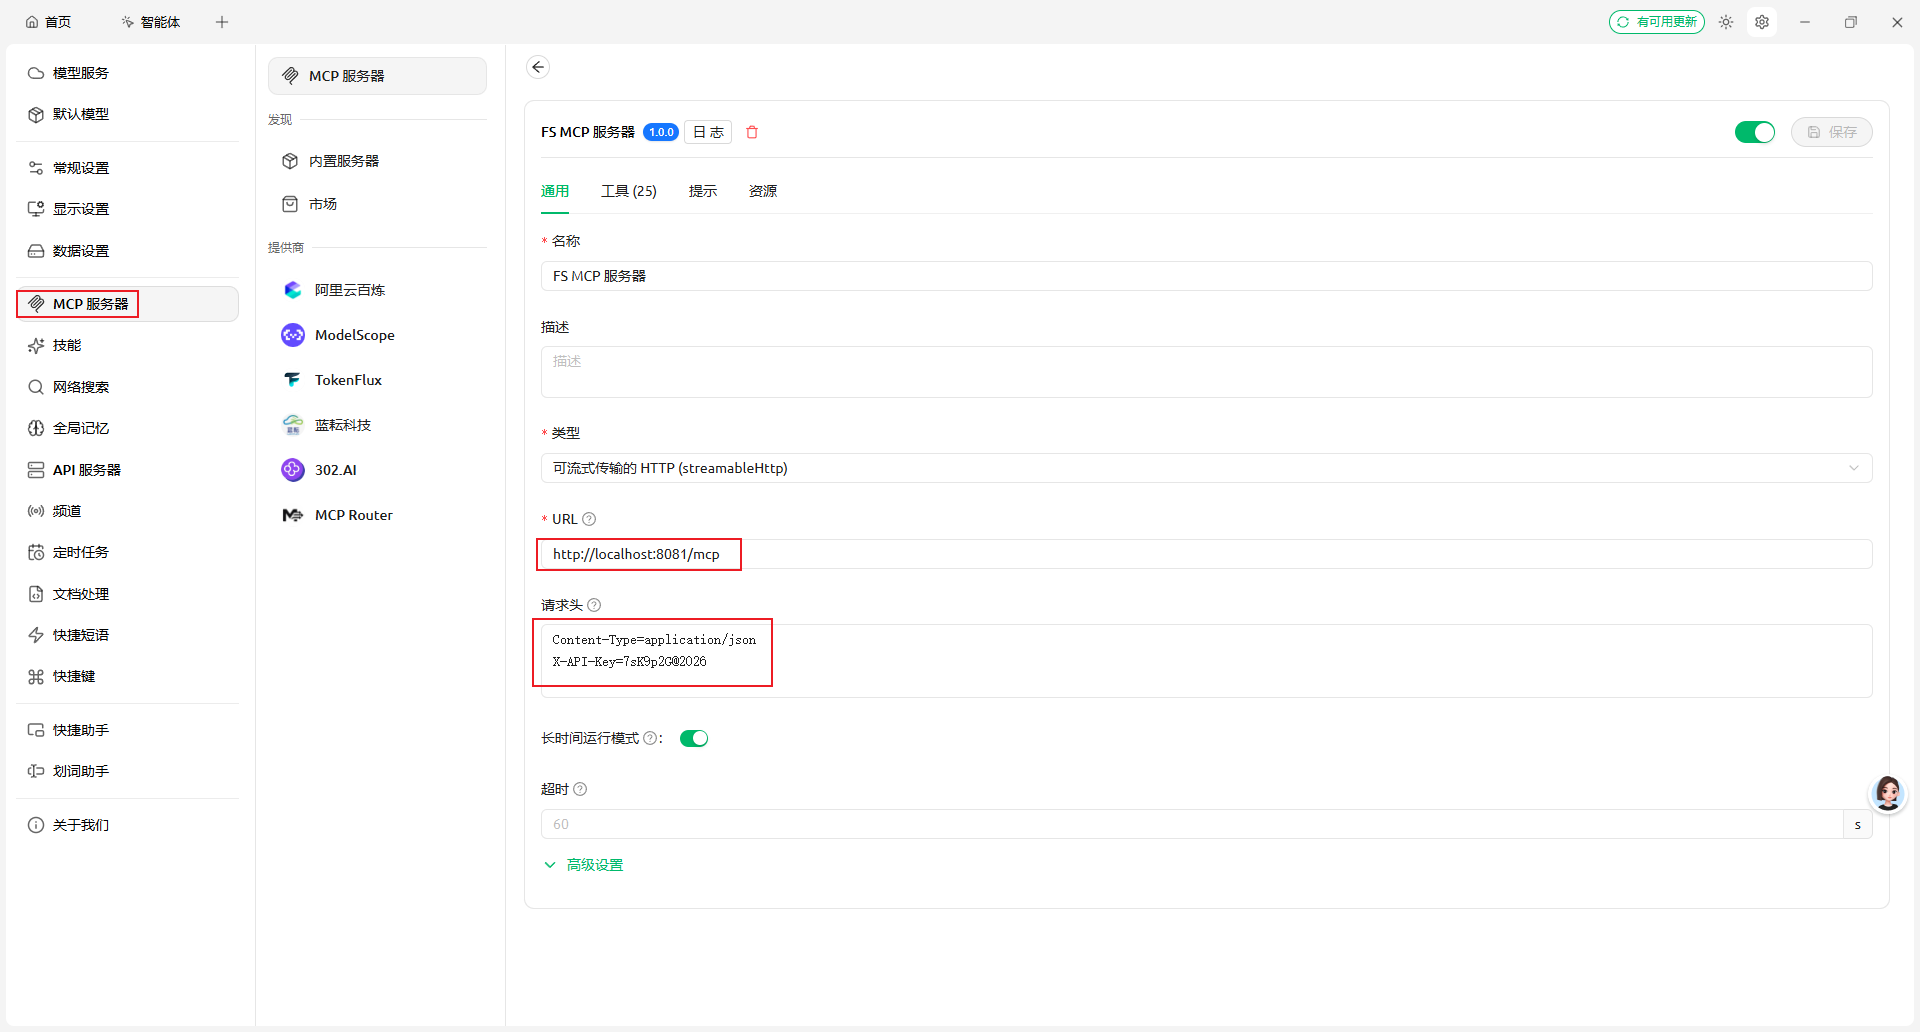
\includegraphics[width=0.9\textwidth]{pics/mcp/cherry-studio-1.png}
	\caption{CherryStudio配置 FS MCP}\label{fig:cherry-studio-1}
\end{figure}
\begin{figure}[h!]
	\centering
	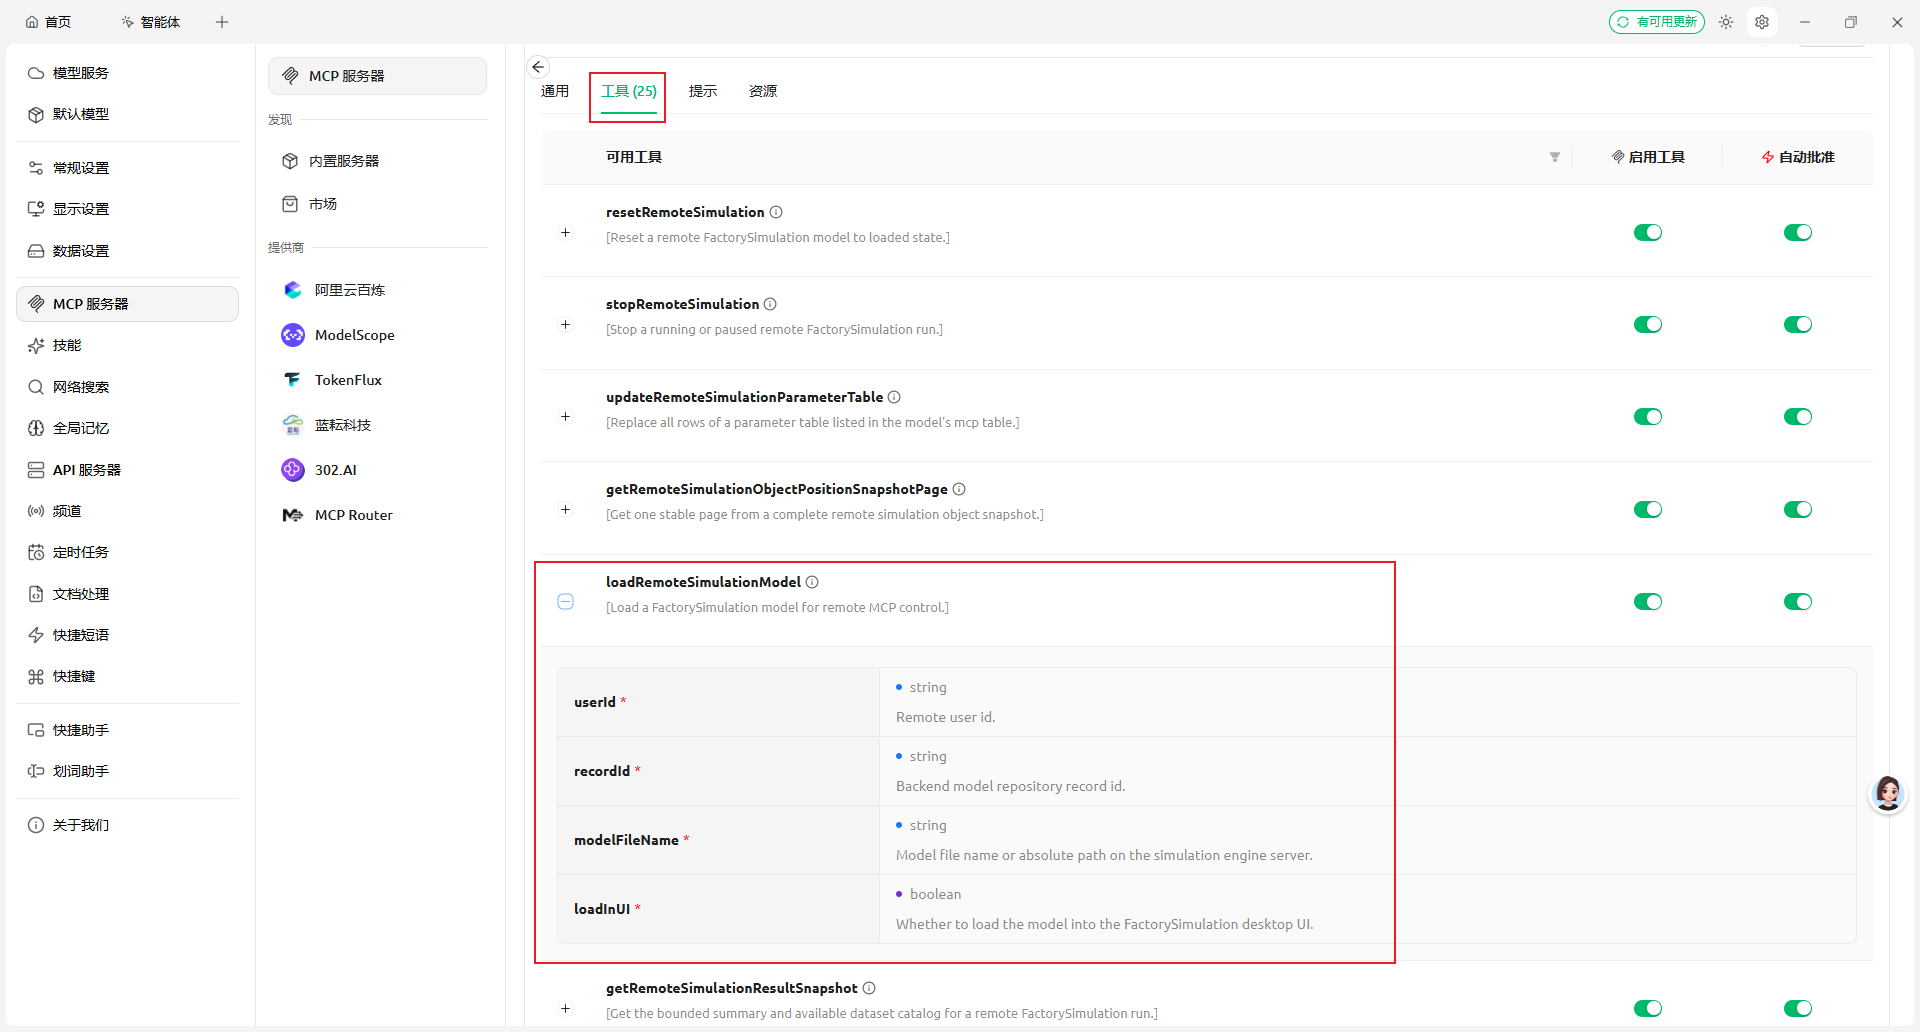
\includegraphics[width=0.9\textwidth]{pics/mcp/cherry-studio-2.png}
	\caption{查看MCP工具}\label{fig:cherry-studio-2}
\end{figure}
\begin{figure}[h!]
	\centering
	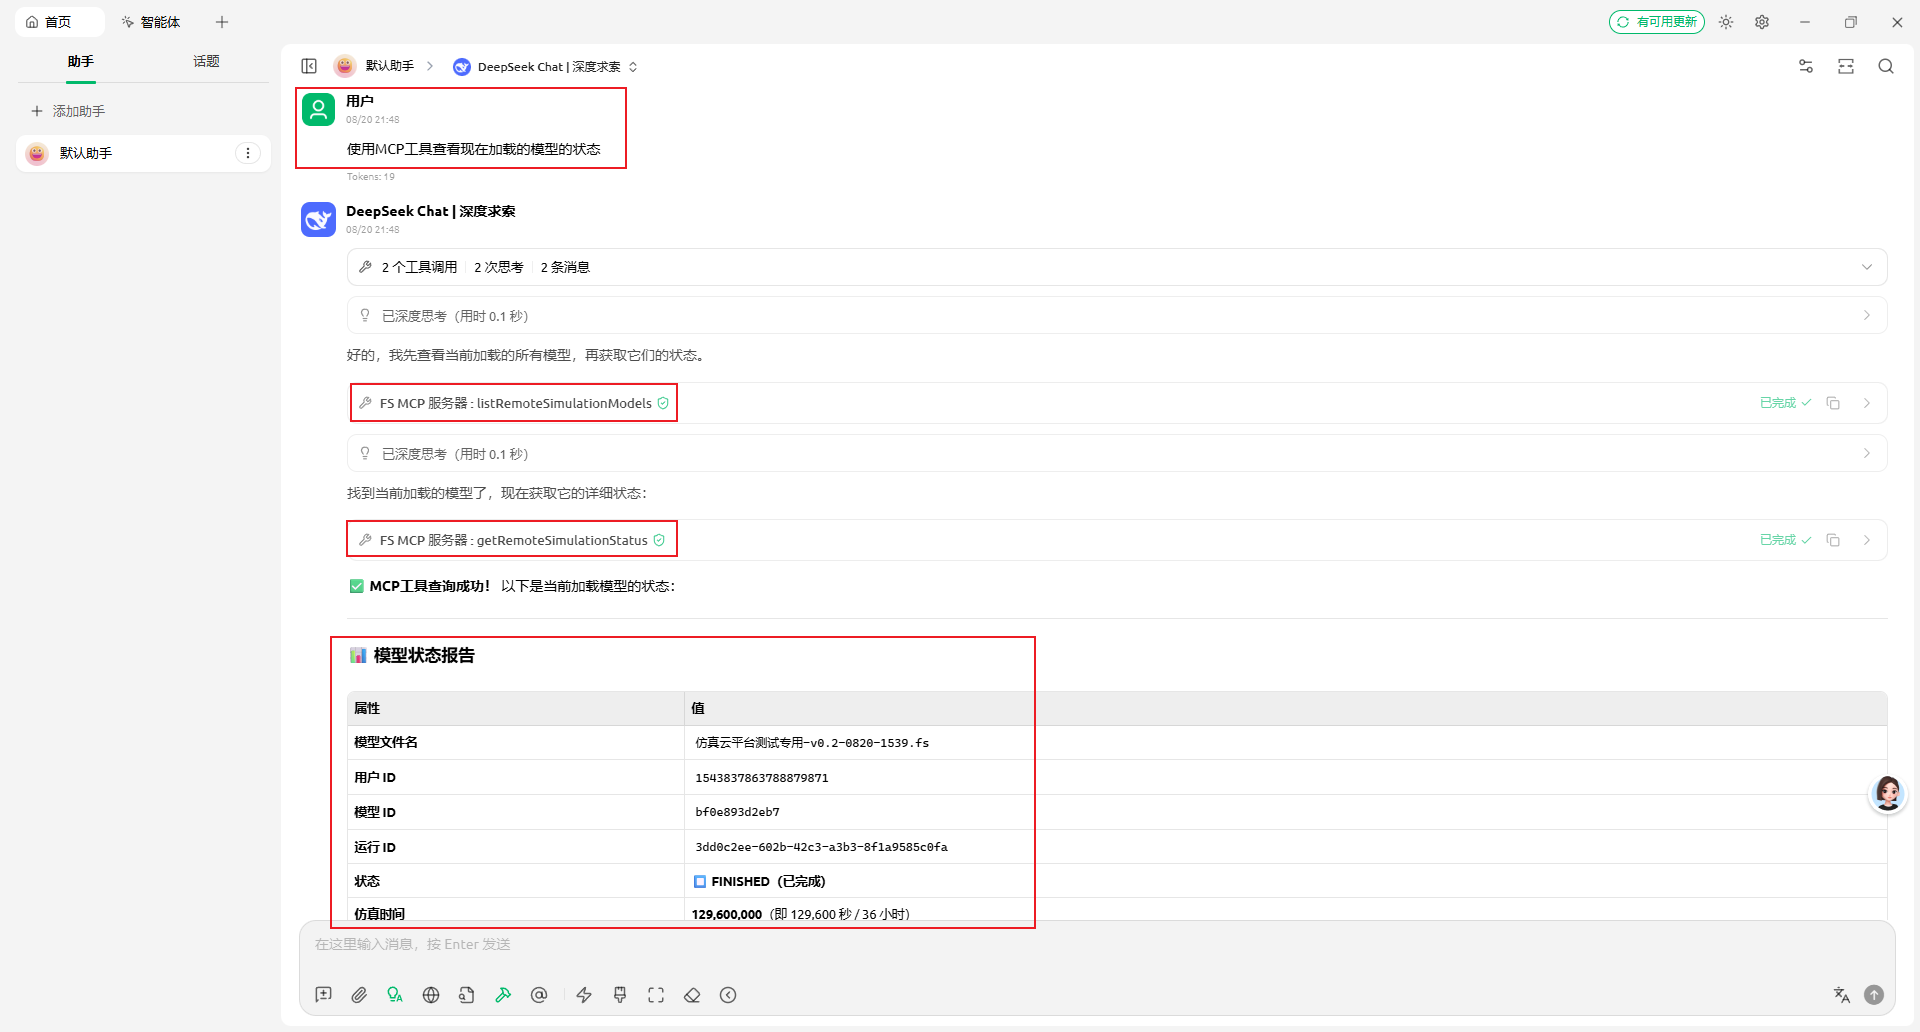
\includegraphics[width=0.9\textwidth]{pics/mcp/cherry-studio-3.png}
	\caption{自然语言提问，LLM自动调用MCP工具}\label{fig:cherry-studio-3}
\end{figure}

\section{附录：MQTTX辅助调试}\label{appendix:mqttx}
\begin{figure}[h!]
	\centering
	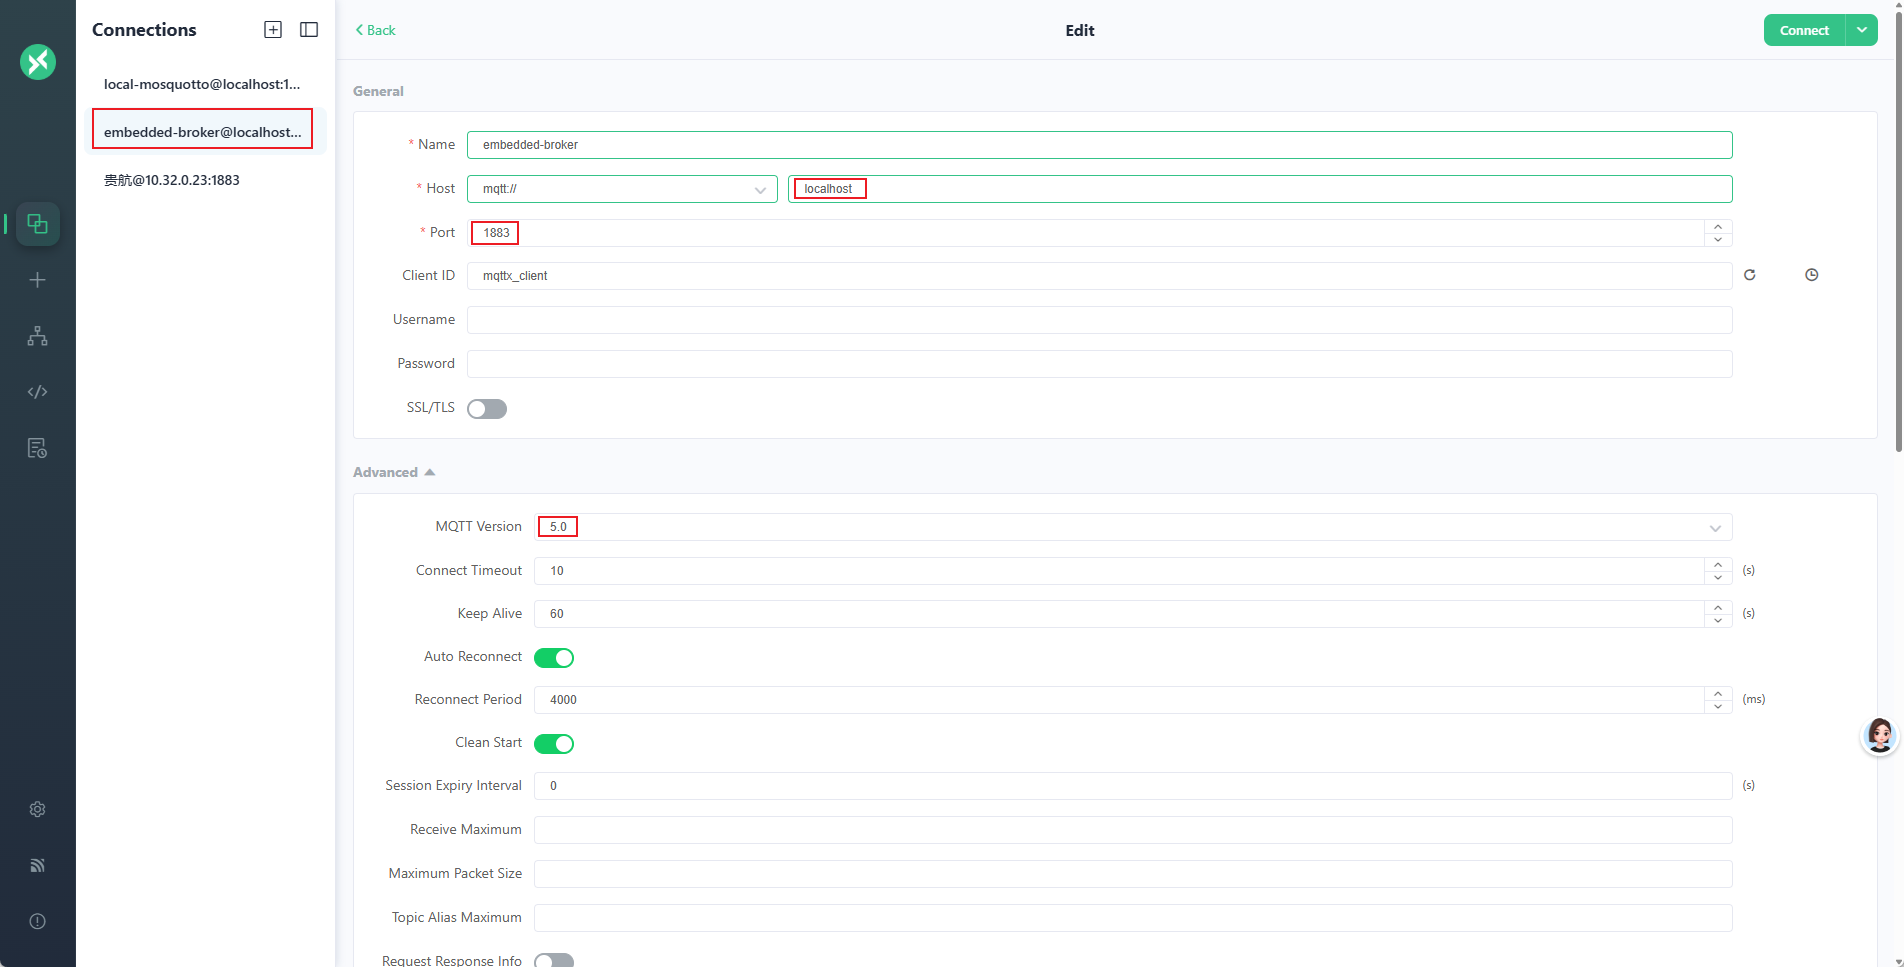
\includegraphics[width=0.9\textwidth]{pics/mcp/mqttx-1.png}
	\caption{MQTTX连接配置}\label{fig:mqttx-1}
\end{figure}
\begin{figure}[h!]
	\centering
	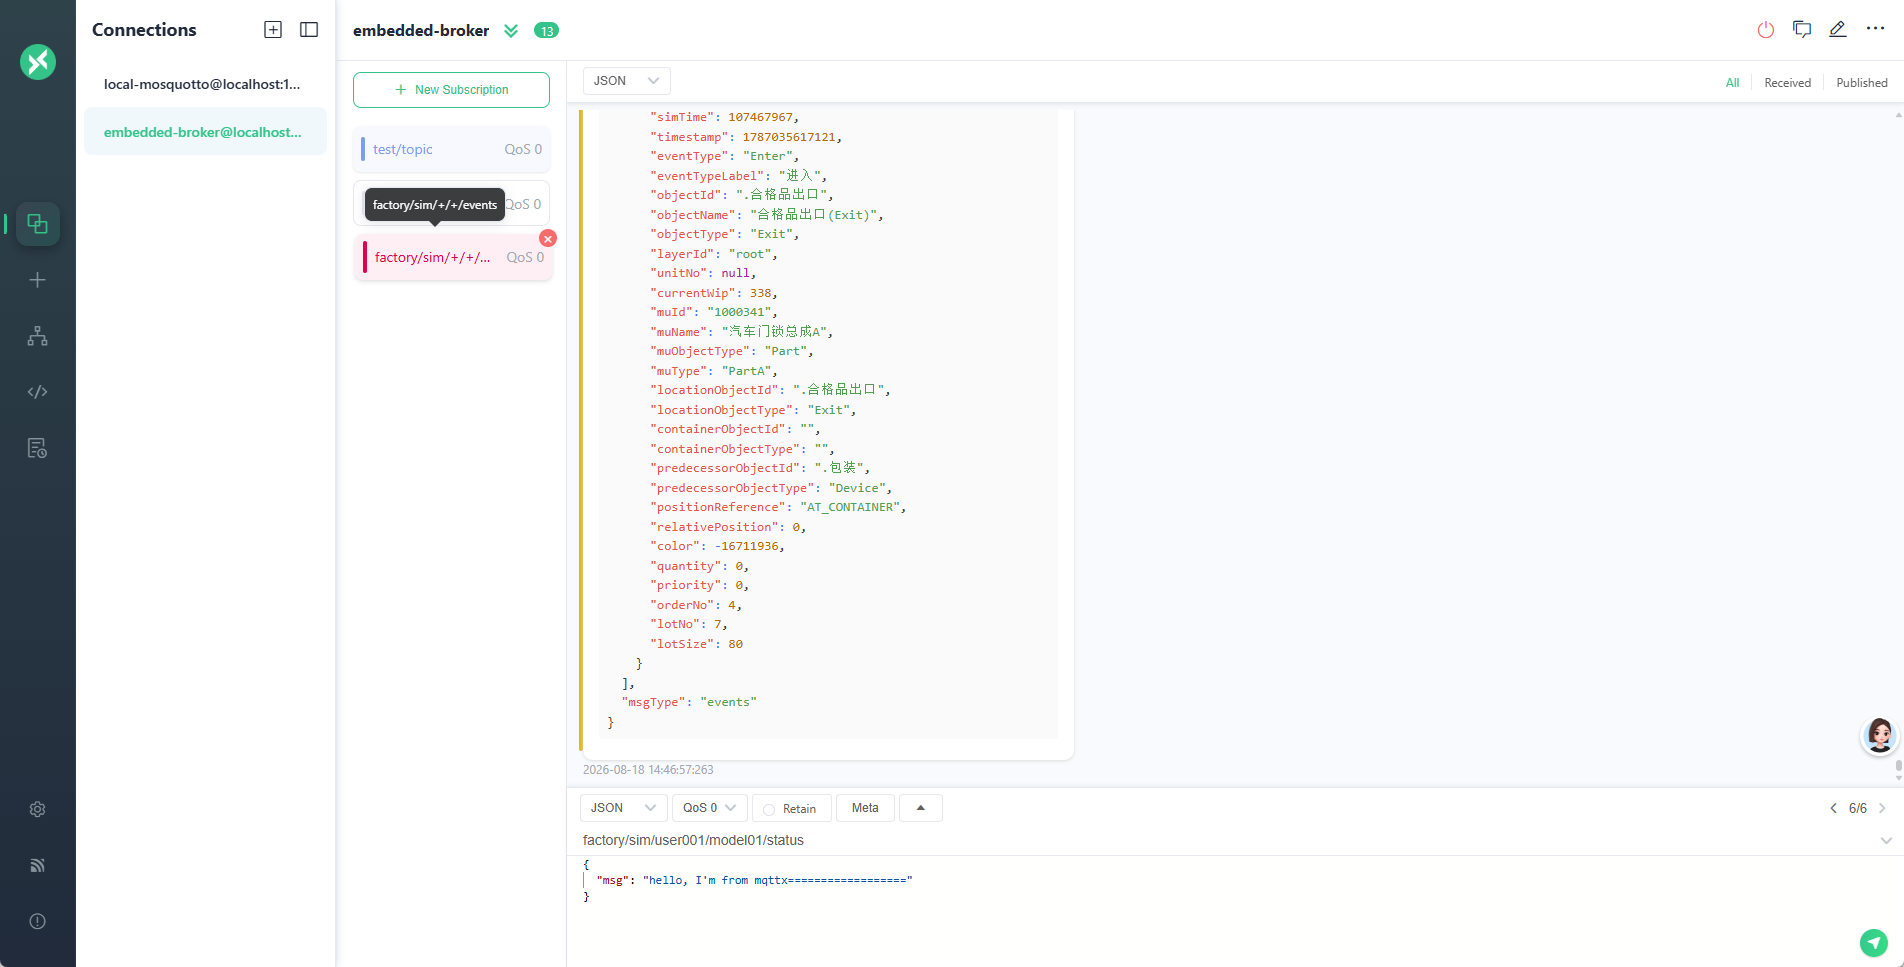
\includegraphics[width=0.9\textwidth]{pics/mcp/mqttx-2.png}
	\caption{MQTTX订阅主题调试}\label{fig:mqttx-2}
\end{figure}
